\chapter{Optimizaciones estructurales}
\label{chap:4}

Un algoritmo con buenos resultados visuales incluye unos costes computacionales asociados. A parte de buscar fotorrealismo y fidelidad gráfica, un motor de renderizado gráfico requiere de mejoras y optimizaciones para alcanzar tiempos competentes.

La importancia de las optimizaciones implementadas en este capítulo no solo se limita a mejorar la productividad de los artistas con mejoras de rendimiento, si no que hace posible la visualización real de escenas que tardarían tiempos del orden de miles de años, reduciendo el enfoque de fuerza bruta a uno más sofisticado.
	
\section{Muestreo por importancia}
\label{sec:mi}

El simple hecho de simular los caminos de los fotones no es eficiente. Se puede buscar una manera para que cada camino cargue con información ''más útil''. Este procedimiento se denomina muestreo por importancia, y es actualmente una línea de investigación en constante desarrollo ya que como se verá a continuación, permite mejoras muy significativas en cuanto al tiempo de convergencia de la imagen final.

Gran parte de la literatura al respecto se resume en las notas de Importance Sampling for Production Rendering\cite{colbert2010importance} donde se repasan todos los fundamentos teóricos del muestreo por importancia. Así pues en este trabajo solo se va a ofrecer una visión generalizada suficiente para entender la implementación realizada en Eleven Renderer.

Esta implementación consta de tres muestreos por importancia distintos: Muestreo por importancia de BRDF, Estimación de Evento Próximo (NEE) y Muestreo por importancia del mapa de entorno.

Algo que todas las técnicas de  muestreo por importancia tienen en común es su funcionamiento primario: Emitir más rayos en las direcciones que más interesan y a su vez, dividir el resultado por la función de distribución de probabilidad (\code{pdf} en adelante). Esto quiere decir que si se emiten el doble de rayos en una dirección que en otra, será necesario dividir este resultado por dos, puesto que se ha recabado el doble de radiación lumínica. Así pues, también se tendrá que multiplicar el resultado menos muestreado por el doble, ya que al muestrear la mitad, se obtiene la mitad de radiación.

Cuando se ha explicado \hyperref[subsec:montecarlo]{la aproximación de la Ecuación de Renderizado} se ha mostrado un denominador $p(\omega _{\text{k}})$ que hasta el momento no ha jugado ningún papel. Este denominador es en efecto la función \code{pdf}.

En la implementación, todo muestreo consiste en una función que genera rayos aleatorios a aquellos lugares donde interesa más muestrear \code{sample()} y la función de distribución de probabilidad apropiada \code{pdf()} derivada de la función de muestreo, que ha de devolver la probabilidad con la que se ha elegido ese camino. Como se verá más adelante, no siempre es fácil derivar esta función de probabilidad cuando se cuenta con una función de muestreo compleja.


\subsection{Muestreo por importancia de Estimación de Evento Próximo (NEE)}
\label{sub:nee}

El renderizado por luz directa es un método por el cual solo se tiene en cuenta la primera interacción del rayo con la escena y se comprueba si dicho punto es visible a los elementos lumínicos. Este método converge muy rápido puesto que solo necesita computar una interacción y el fotón recibe información directamente de la luz sin tener que desperdiciar fotones que acaben en zonas oscuras, pero carece del fotorrealismo que ofrece la iluminación global o luz indirecta, puesto no tiene en cuenta la luz reflejada en otros elementos no emisivos.

El muestreo por importancia de Estimación de Evento Próximo trata de juntar estos dos métodos: La iluminación directa y la indirecta. De esta manera, la parte expuesta directamente a elementos lumínicos convergerá rápidamente, además de las partes afectadas por la iluminación global, que lo harán también. Un añadido de este método es la posibilidad de computar la iluminación dada por luces de punto.

Las luces de punto consisten en un punto en el espacio infinitamente pequeño que emite luz de manera uniforme hacia todos los lados. Sin la implementación de la estimación de evento próximo, nunca se recibiría información lumínica de estas luces ya que al ser infinitamente pequeñas no sérian alcanzadas por los caminos. No solo eso, NEE también permite una mejor convergencia en las luces de menor tamaño, puesto que originalmente, las luces tienen menos probabilidades de ser alcanzadas cuanto menor sea su área.

En el caso de Eleven Renderer, una nueva función \code{pointLight} en \autoref{cod:pointlight} es utilizada. Esta función calcula la luz directa de los puntos de luz. De forma resumida, se elige un punto de luz aleatorio, se toma como radiación inicial el atributo \code{radiance} para dicho punto de luz y se atenúa cuadráticamente con la distancia entre la luz y el punto a sombrear. Este procedimiento es realmente intuitivo si se trata la luz como una esfera y la radiación emitida como el área de dicha esfera. Finalmente se aplica la función BRDF para la dirección a la luz y el coseno con la normal. También es necesario un paso por el que se comprueba si dicho punto es visible por la luz o está obstruído por un objeto, para ello se traza un rayo hasta la luz y se comprueba si interseca con algún triángulo.

La función \code{pdf} se obtiene a partir del número de luces. Por otro lado, hay que hacer un cambio de dominio, ya que hasta el momento la función \code{pdf} solo tiene en cuenta la luz de las luces y no toda la luz de la escena. Este cambio de dominio se hace dividiendo entre el área de media esfera \code{2.0 * PI}, ya que es el área del que se mide la radiación entrante.

\begin{minipage}[c]{0.95\textwidth}
\begin{lstlisting}[label={cod:pointlight}, caption={Código de iluminación por luces puntuales}]
	
	__device__ Vector3 pointLight(Ray ray, HitData hitdata, dev_Scene* scene, Vector3 point, float& pdf, float r1) {

		if (scene->pointLightCount <= 0) {
			pdf = 0;
			return Vector3::Zero();
		}

		pdf = ((float)scene->pointLightCount) / (2.0 * PI);

		// Retrieve a random light
		PointLight light = scene->pointLights[(int)(scene->pointLightCount * r1)];
		
		Vector3 newDir = (light.position - point).normalized();
		
		float dist = (light.position - point).length();

		// Test if the point is visible from the light
		Ray shadowRay(point + newDir * 0.000001, newDir);
		Hit shadowHit = throwRay(shadowRay, scene);
		float shadowDist = (shadowHit.position - point).length();

		if (shadowHit.valid && shadowDist < dist)
			return Vector3();

		// Quadratic attenuation
		Vector3 pointLightValue = (light.radiance / (dist * dist));

		Vector3 brdfDisney = DisneyEval(ray, hitdata, newDir);

		return pointLightValue * brdfDisney * abs(Vector3::dot(newDir, hitdata.normal)) / pdf;
	}
	
\end{lstlisting}
\end{minipage}

\subsection{Muestreo por importancia de entorno}
	
Anteriormente se ha descrito cómo la iluminación HDRI permite resultados visualmente complejos de manera sencilla, simplemente con una imagen de alta profundidad de color. Este método, por otra parte, también cuenta con inconvenientes. 

Antes de aplicar cualquier tipo de optimización a este método de iluminación, se estaba trazando un rayo de manera ingenua, recibiendo el color de la imagen a partir de las coordenadas esféricas asumiendo una esfera de radio infinito. Para imágenes homogéneas con luminosidad similar en cada píxel. Este método funciona muy bien, pero la mayoría de estas imágenes HDRI consisten en un paisaje con componentes lumínicos condensados como el sol, que actúa como principal fuente de luz.

Esta situación plantea un problema, y es que los focos de luz como puede ser el sol, concentran un gran porcentaje de luminosidad, mientras que el resto de la imagen no. Esto implica que pocas veces se va a recibir información del sol, lo que va a resultar en ''fireflies'' (píxeles que cargan una gran radiación lumínica, por la naturaleza aleatoria de las muestras). En la \autoref{fig:hdriisoff} se muestra este fenómeno.

La forma de enfrentar este problema es igual que el resto de muestreo por importancia: Trazar más rayos a los píxeles más luminosos, ya que serán aquellos que más información aporten a la escena. En la implementación se activa y desactiva con la definición \code{\#define HDRIIS = true/false}

\begin{figure}[H]
\label{fig:hdriis}
	\centering
  \begin{subfigure}[b]{0.4\textwidth}
	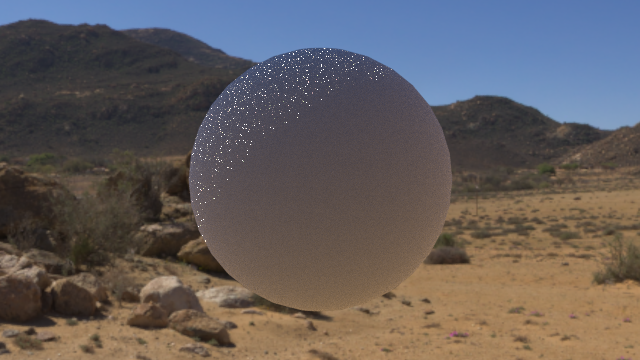
\includegraphics[width=\textwidth]{hdriisoff}
	\caption{HDRIIS = false}
	\label{fig:hdriisoff}
  \end{subfigure}
  \hfill
  \begin{subfigure}[b]{0.4\textwidth}
	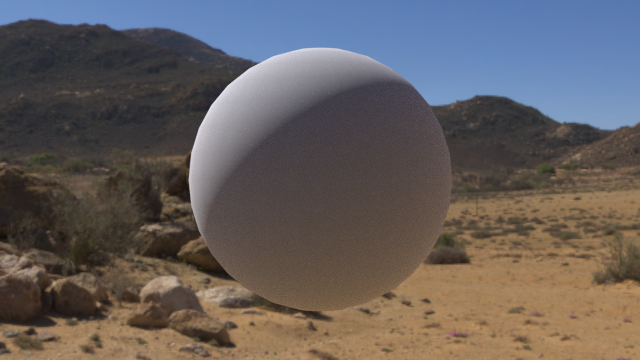
\includegraphics[width=\textwidth]{hdriison}
	\caption{HDRIIS = true}
	\label{fig:hdriison}
  \end{subfigure}
\end{figure}

La implementación de este tipo de muestreo por importancia no es trivial. Las imágenes HDRI utilizadas normalmente en la industria cinematográfica suelen contar con resoluciones extremas (\~8K) y son del orden de millones de píxeles. La búsqueda de los píxeles más brillantes y la asignación de su probabilidad de ser elegidos requerirá de un preprocesamiento previo que facilite dicha búsqueda.

El planteamiento general para este método consiste en precomputar un array del tamaño del número total de píxeles de la imagen HDRI, en el que cada elemento cuente con la iluminación acumulada normalizada hasta el momento de cada píxel \autoref{fig:CDF}.
La función que determina la iluminación de un píxel viene dada por la respuesta logarítmica media de los bastones y conos de los ojos para cada longitud de onda, pero para simplificar se utilizará la suma de cada componente de color. Este array, a efectos prácticos contiene la función de distribución acumulativa discreta normalizada (CDF) y, como está ordenado, es posible hacer búsquedas binarias, las cuales cuentan con una complejidad logarítmica (aproximadamente 25 iteraciones de búsqueda para una imagen de 8K de resolución).

En el código desarrollado para la implementación \autoref{cod:generatecdf}, el primer bucle anidado computa la radiación total de la imagen. Este valor se usa para posteriormente normalizar el \code{CDF} a la vez que se calcula en el segundo bucle anidado.


\begin{figure}[H]
    \centering
	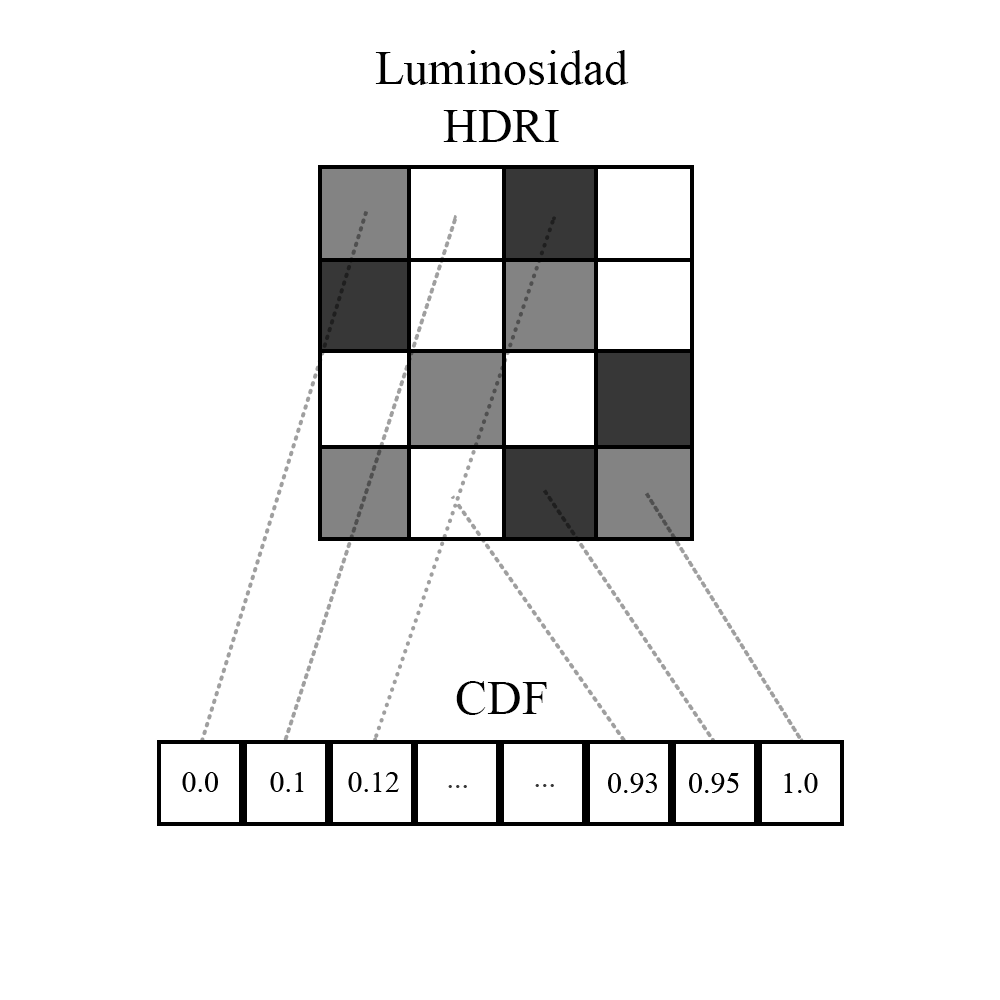
\includegraphics[width=0.5\textwidth]{CDF}
	\caption{Función de distribución acumulada}
	\label{fig:CDF}
\end{figure}

\begin{minipage}[c]{0.95\textwidth}
\begin{lstlisting}[label={cod:generatecdf}, caption={Generación de la función de distribución acumulada}]
	
	__host__ __device__ inline void generateCDF() {

		int c = 0;
		radianceSum = 0;
		cdf[0] = 0;

		// Total radiance of the HDRI
		for (int j = 0; j < texture.height; j++) {
			for (int i = 0; i < texture.width; i++) {
				Vector3 data = texture.getValueFromCoordinates(i, j);
				radianceSum += data.x + data.y + data.z;
			}
		}
		// CDF calculation
		for (int j = 0; j < texture.height; j++) {
			for (int i = 0; i < texture.width; i++) {
				Vector3 data = texture.getValueFromCoordinates(i, j);
				cdf[c + 1] = cdf[c] + (data.x + data.y + data.z) / radianceSum;
				c++;
			}
		}
	}
	
\end{lstlisting}
\end{minipage}

La función de cálculo de CDF implementada realiza dos simplificaciones en comparación al método propuesto en la literatura. En primer lugar simplifica la dimensionalidad del array CDF en una sola dimensión (en la literatura se utiliza una segunda dimensión que acumula un sumatorio de radiancia con el fin de acelerar la búsqueda). En segundo lugar, realiza el muestreo por importancia utilizando las coordenadas de las texturas en píxeles y no en coordenadas esféricas (normalmente se muestrea a través de las coordenadas esféricas con el fin de evitar deformaciones en los polos). Se ha determinado que este método modificado es más intuitivo para una versión preeliminar, aunque queda sujeto a cambios en posteriores versiones. 

Si se quiere obtener un píxel de manera aleatoria proporcional a su iluminación, bastará con buscar en el CDF el intervalo que comprende el valor aleatorio dado. Esta operación de búsqueda también tiene coste logarítmico, ya que es una versión ligeramente modificada de la búsqueda binaria corriente. Este tipo de búsqueda está disponible en la librería estándar de C++ \code{std::lower\_bound}, pero se ha realizado la implementación manual para CUDA. Esta acción es realizada por la función \code{sample}, que a partir de un número aleatorio, devolverá un píxel del HDRI, siendo los más brillantes los más comunes.

\begin{minipage}[c]{0.95\textwidth}
\begin{lstlisting}[label={cod:hdriis}, caption={Código para el muestreo por importancia de entorno y función auxiliar}]
	
	// Lower_bound kinda function.
	__host__ __device__ int binarySearch(float* arr, float value, int length) {

		int from = 0;
		int to = length - 1;

		while (to - from > 0) {
			int m = from + (to - from) / 2;
			if (value == arr[m]) return m;
			if (value < arr[m])	to = m - 1;
			if (value > arr[m]) from = m + 1;
		}
		return to;
	}
	
	__host__ __device__ Vector3 sample(float r1) {
		// Returns position in the array
		int count = binarySearch(cdf, r1, texture.width * texture.height);

		int x = count % texture.width;
		int y = count / texture.width;

		return Vector3(x, y, 0);
	}
	
	__host__ __device__ float pdf(int x, int y) {

		Vector3 dv = texture.getValueFromCoordinates(x, y);
		float theta = (((float)y / (float)texture.height)) * PI;

		// Semisphere area
		return ((dv.x + dv.y + dv.z) / radianceSum) * texture.width * texture.height / (2.0 * PI * sin(theta));
	}
	
\end{lstlisting}
\end{minipage}

Por último, como se está muestreando en mayor proporción los píxeles más brillantes, es necesario ofrecer una función \code{pdf} apropiada. La intuición sugiere que la posibilidad de elegir un píxel entre el resto es la iluminación de dicho píxel dividida entre la suma de toda la iluminación del HDRI \code{(dv.x + dv.y + dv.z) / radianceSum}. No obstante aún faltan matices. Puesto que se está calculando la luz de un solo píxel en vez de toda la imagen, es necesario multiplicar el \code{pdf} por el número total de píxeles de la imagen \code{texture.width * texture.height}. Además, se aplica el cambio de dominio explicado en \autoref{sub:nee}. El cálculo de esta función \code{pdf} es una extensión del cálculo en NEE, ya que se está considerando un HDRI como un conjunto de luces.

Debido a la deformación de una imagen plana al ser transladada a una superficie esférica, se va a observar un mayor número de muestras en los polos. Este mayor número de muestras en los polos se podría reducir en la función de CDF (es una de las simplificaciones realizadas), pero en vez de eso se añade un término adicional \code{sin(theta)} que reduce la intensidad de los píxeles más cercanos a los polos.


\subsection{Muestreo por importancia de BRDF}

La función BRDF aporta distintas intensidades lumínicas dependiendo de la dirección entrante y la dirección saliente, por lo que sería mucho más óptimo lanzar más rayos a los sitios en los que esta función sea mayor e ignorar aquellos sitios donde no se aporte mucha información al resultado final.

Un ejemplo que ayuda a visualizar este caso son los materiales perfectamente reflectantes (espejos). Los materiales reflectantes tienen un valor \code{BRDF = 1} para todo rayo entrante simétrico al saliente con la normal como eje de reflexión. Para el resto de direcciones el valor será 0. Por esta razón no tiene sentido emitir rayos aleatorios donde se conozca que el resultado del BRDF será 0.

Así pues, la función \code{sample} deberá emitir más muestrás allá donde la función \code{brdf} sea mayor. La implementación utilizada contiene una función \code{DisneySample} que se encarga de esto. Un análisis más detallado de la derivación de esta función a partir de las ecuaciones del shader de Disney se puede encontrar en la implementación de este en el motor de renderizado Autodesk Arnold \cite{arnoldimplementation}

A partir de esta función de muestreo, el autor de la implementación utilizada ofrece también la función \code{pdf}. Cabe decir que ambas funciones han sido modificadas y adaptadas para la implementación de Eleven Renderer, eliminando por ejemplo los términos de transmisión en ambas funciones.

Gracias a este muestreo, es posible renderizar materiales metálicos. Anteriormente, la convergencia de estos materiales era lenta e impráctica como se aprecia en la \autoref{fig:brdfisoff} incluso para un número de muestras muy elevado. Tras aplicar el muestreo por importancia el resultado de los materiales metálicos es mucho más nítido \autoref{fig:brdfison}.

\begin{figure}[H]
	\label{fig:brdfis}
	\centering
  \begin{subfigure}[b]{0.45\textwidth}
	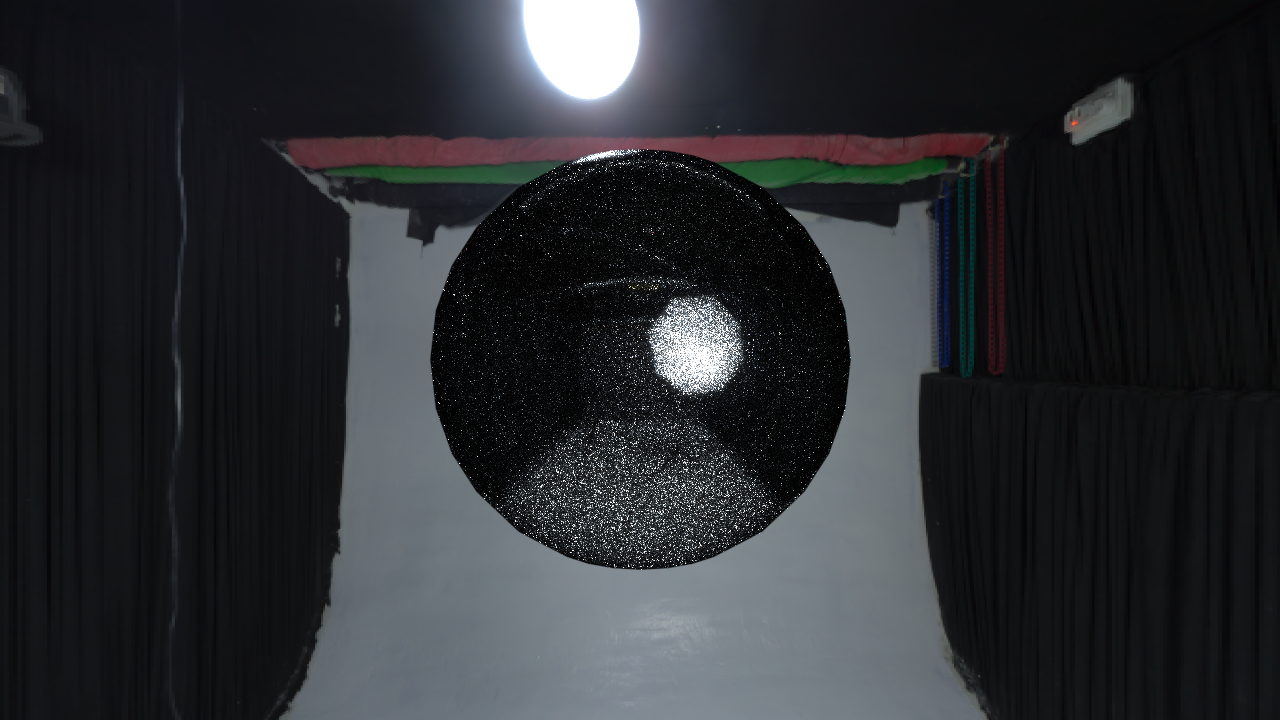
\includegraphics[width=\textwidth]{brdfisoff}
	\caption{Muestreo uniforme}
	\label{fig:brdfisoff}
  \end{subfigure}
  \hfill
  \begin{subfigure}[b]{0.45\textwidth}
	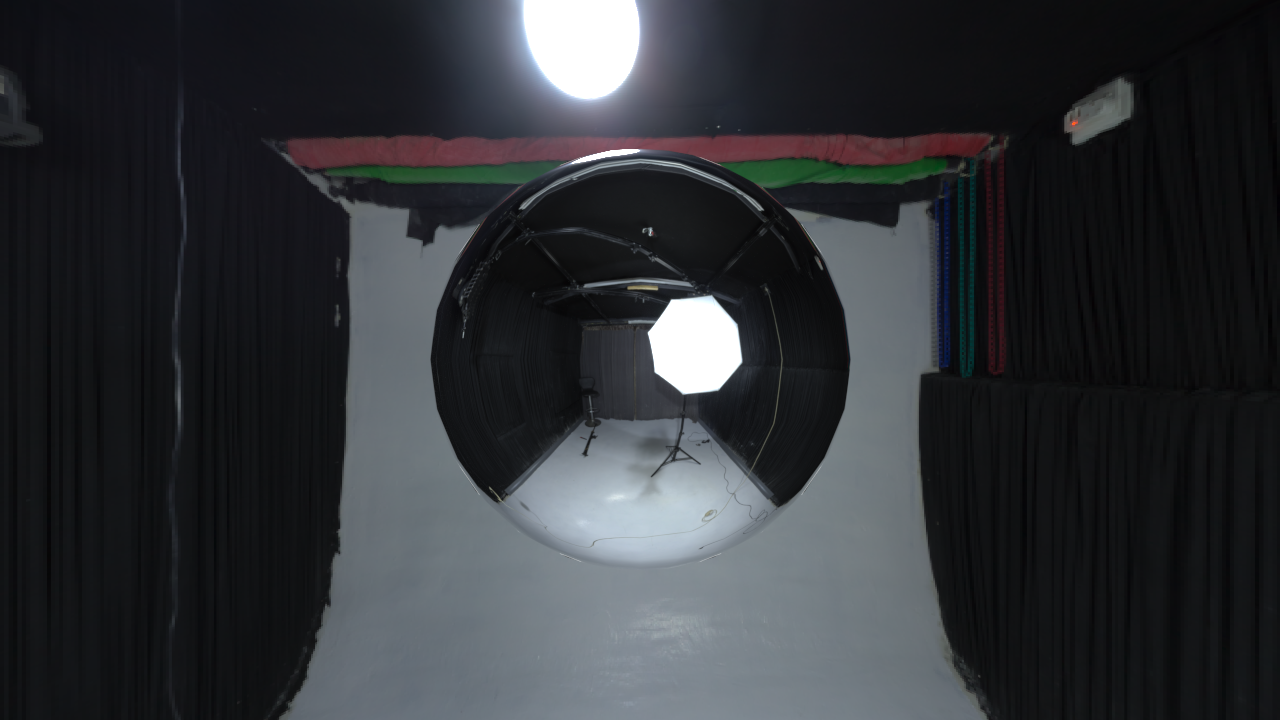
\includegraphics[width=\textwidth]{brdfison}
	\caption{Muestreo por importancia}
	\label{fig:brdfison}
  \end{subfigure}
  \caption{Diferencias entre distintos muestreos}
\end{figure}

\subsection{Muestreo por importancia múltiple}

El muestreo por importancia es una herramienta que mejora considerablemente los tiempos de convergencia en determinados escenarios. Como se ha visto hay distintos tipos de muestreos, con distintos puntos fuertes en diversos escenarios. La verdadera utilidad de estos es elegir el muestreo correcto para cada situación. En 1975 se propone una técnica conocida como MIS (Multiple Importance Sampling) \cite{veach1995optimally}. Esta técnica evalúa todas las funciones de muestreo para cada intersección y da mayor importancia con un escalar a aquellas funciones que proporcionen mayor información de la escena.

El cálculo de este escalar se realiza a través de una heurística y debe tener una propiedad esencial: $\sum{w(M_i)} = 1$. En primer lugar el enfoque más ingénuo es utilizar escalares constantes que sumen 1. Esto garantizará el uso de todos los métodos de muestreo de manera igualitaria pero con el inconveniente de no aportar ningún tipo de ventaja a los métodos más relevantes. 

Por otro lado, una heurística más acertada e intuitiva es ponderar cada método a partir de su \code{pdf}. Esto quiere decir que será más eficiente dar más importancia al método con mayor \code{pdf}. Con dos tipos de muestreo diferentes $M_1, M_2$ quedaría así: $w(M_1) = \frac{pdf1}{pdf1 + pdf2}, w(M_2) = \frac{pdf2}{pdf1 + pdf2}$. Se puede comprobar algebraicamente que la suma de ambos pesos es uno.


En los motores de producción se utiliza por lo general una heurística llamada Power Heuristic debido a que Veach \cite{veach1995optimally} la determina empíricamente mejor. Para Eleven Renderer se ha utilizado heurística de ponderación por \code{pdf} con el fin de ser más comprensivo. En futuras versiones más orientadas a producción se procederá a cambiar esta heurística.

\section{Estructuras de aceleración}
\label{BVH}
	
Pese a que este punto cuenta con un nombre genérico, las estructuras de aceleración en el ámbito del renderizado por trazado de rayos hacen referencia a la interacción específica entre geometrías tridimensionales y los rayos generados por la cámara. La intersección Rayo-Triángulo no es en sí una operación demandante a nivel computacional, pero la mayoría de las escenas suelen contar con complejas geometrías del orden de miles de millones de triángulos.

El enfoque más ingenuo y utilizado hasta el momento en este motor de renderizado consiste en evaluar triángulo a triángulo si intersecciona con el rayo dado. Así pues, se observa que es posible reducir el número de comprobaciones de intersecciones aplicando una jerarquía espacial a los triángulos, que descarte parte de ellos para cada interacción, reduciendo así considerablemente el número de operaciones.

Existen diversas formas de estructurar estas jerarquías. Nombrando las más conocidas: Octrees, k-d tree y BVH. En esta implementación se ha usado BVH puesto que se considera que tiene muy buenos resultados.

BVH es acrónimo de "Bounding Volume Hierarchy", traducido como jerarquía del volumen delimitador y consiste en un árbol binario de profundidad definida en el que cada nodo cuenta con un el prisma rectangular que delimita un conjunto de triángulos (en la práctica este prisma consiste en dos puntos en el espacio). Cada nodo interior tiene dos hijos y cada hijo, el volumen delimitador del subconjunto disjunto de los triángulos del nodo padre. Los nodos hoja cuentan con el volumen delimitador y con una lista de los triángulos que contienen, como se muestra en la \autoref{fig:bvhdiagram}.

\begin{figure}[H]
    \centering
	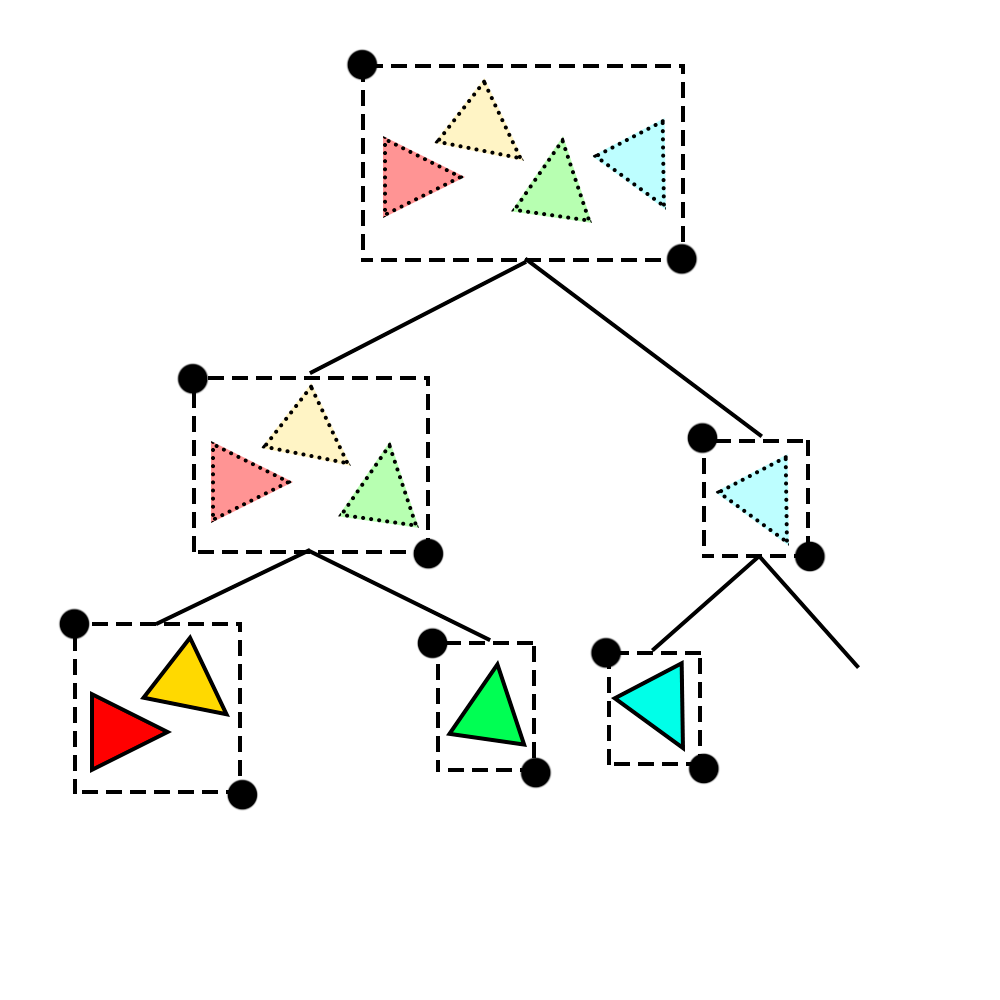
\includegraphics[width=0.5\textwidth]{BVH}
	\caption{División BVH}
	\label{fig:bvhdiagram}
\end{figure}

De esta manera será posible descartar gran parte de los triángulos comprobando los volúmenes por los cuales interseccionan los rayos.

Esta nueva estructura de datos BVH cuenta con dos operaciones fundamentales: La operación de creación \code{build} y la operación de recorrido \code{transverse}. La operación de creación será necesaria solo una vez al principio de cada renderizado de escena y podrá ser realizada en la CPU para mayor simplicidad. La operación de recorrido sin embargo será ejecutada cada vez que se quiera comprobar la interacción Rayo-Triángulo.

El algoritmo empleado es una interpretación del libro PBRT, pero difiere en varios detalles. Pharr et al. \cite{pharr2016physically} almacena un solo triángulo por cada nodo hoja, a diferencia del código implementado en Eleven Renderer, donde hay una profundidad máxima definida como \code{BVH\_DEPTH}, y los nodos hojas almacenan los índices de uno o varios triángulos. 

\subsection{Operación de generación de BVH (CPU)}

La operación de generación parte de la generación recursiva de un árbol binario por profundidad, añadiendo información adicional a los nodos. Esta operación queda definida en \autoref{cod:generatebvh}

\begin{enumerate}
	
\item Para cada nodo que contiene un conjunto de triángulos, se calcula el volumen delimitador. Este volumen viene dado por el vértice menor y mayor del volumen \code{b1, b2}. 
Los delimitadores son dos puntos que representan el volumen que contiene una geometría. El cálculo de estos se hace cogiendo las coordenadas mínimas y máximas por cada dimensión. Véase \autoref{cod:bounds}

\item Se separa el conjunto de triángulos en dos subconjuntos disjuntos. El cómo se divide este conjunto se delega a la función \code{divideSAH()}, que hará uso de la \hyperref[sub:sah]{heurística de superficie de área} para decidir qué triángulos van a cada subconjunto. Distintas funciones de división de triángulos pueden ser usadas en este punto.

\item Finalmente se aplica recursión para los hijos generados en caso de residir en un nodo interior, o se termina la recursión y se almacenan los índices \code{from} y \code{to} de los triángulos que estos contienen en caso de ser un nodo hoja.

\end{enumerate}

\begin{minipage}[c]{0.95\textwidth}
	\begin{lstlisting}[label={cod:bounds}, caption={Cálculo de delimitadores}]

	static void bounds(Tri tri, Vector3& b1, Vector3& b2) {

		b1.x = minf(tri.vertices[0].x, minf(tri.vertices[1].x, tri.vertices[2].x));
		b1.y = minf(tri.vertices[0].y, minf(tri.vertices[1].y, tri.vertices[2].y));
		b1.z = minf(tri.vertices[0].z, minf(tri.vertices[1].z, tri.vertices[2].z));

		b2.x = maxf(tri.vertices[0].x, maxf(tri.vertices[1].x, tri.vertices[2].x));
		b2.y = maxf(tri.vertices[0].y, maxf(tri.vertices[1].y, tri.vertices[2].y));
		b2.z = maxf(tri.vertices[0].z, maxf(tri.vertices[1].z, tri.vertices[2].z));
	}
	
\end{lstlisting}
\end{minipage}

\begin{minipage}[c]{0.95\textwidth}
\begin{lstlisting}[label={cod:generatebvh}, caption={Generación recursiva del árbol BVH}]
	
	void buildAux(int depth, std::vector<BVHTri>* _tris) {

		Vector3 b1, b2;

		if (depth == 0)
			totalTris = _tris->size();

		if(depth == 7)
			printf("\rAllocated tris: %d / %d, %d%%", allocatedTris, totalTris, (100 * allocatedTris) / totalTris);

		bounds(_tris, b1, b2);

		if (depth == DEPTH) {

			nodes[nodeIdx++] = Node(nodeIdx, b1, b2, triIdx, triIdx + _tris->size(), depth);

			for (int i = 0; i < _tris->size(); i++)
				triIndices[triIdx++] = _tris->at(i).index;

			allocatedTris += _tris->size();
		}
		else {

			nodes[nodeIdx++] = Node(nodeIdx, b1, b2, 0, 0, depth);

			std::vector<BVHTri>* trisLeft = new std::vector<BVHTri>();
			std::vector<BVHTri>* trisRight = new std::vector<BVHTri>();

			divideSAH(_tris, trisLeft, trisRight);

			buildAux(depth + 1, trisLeft);
			buildAux(depth + 1, trisRight);

			trisLeft->clear();
			trisRight->clear();

			delete trisLeft;
			delete trisRight;
		}
	}
	
\end{lstlisting}
\end{minipage}

Una duda que puede surgir es cómo se almacenan los triángulos de manera eficiente en estos árboles, ya que almacenar tantas listas como nodos hoja hay, añade una fuerte penalización en términos de memoria. Aquí es donde entran en juego los índices \code{from} y \code{to} mencionados anteriormente. Se hace uso de una lista de ordenación de triángulos denominada \code{triIndices}, la cual contiene índices de los triángulos en la lista original ordenados por nodos \autoref{fig:triindices}. Los nodo hoja tendrán pues dos índices indicando desde qué índice (\code{from}) hasta qué índice (\code{to}) es necesario leer de manera inclusiva en esta lista para recuperar los triángulos almacenados por dicho nodo.

\begin{figure}[H]
    \centering
	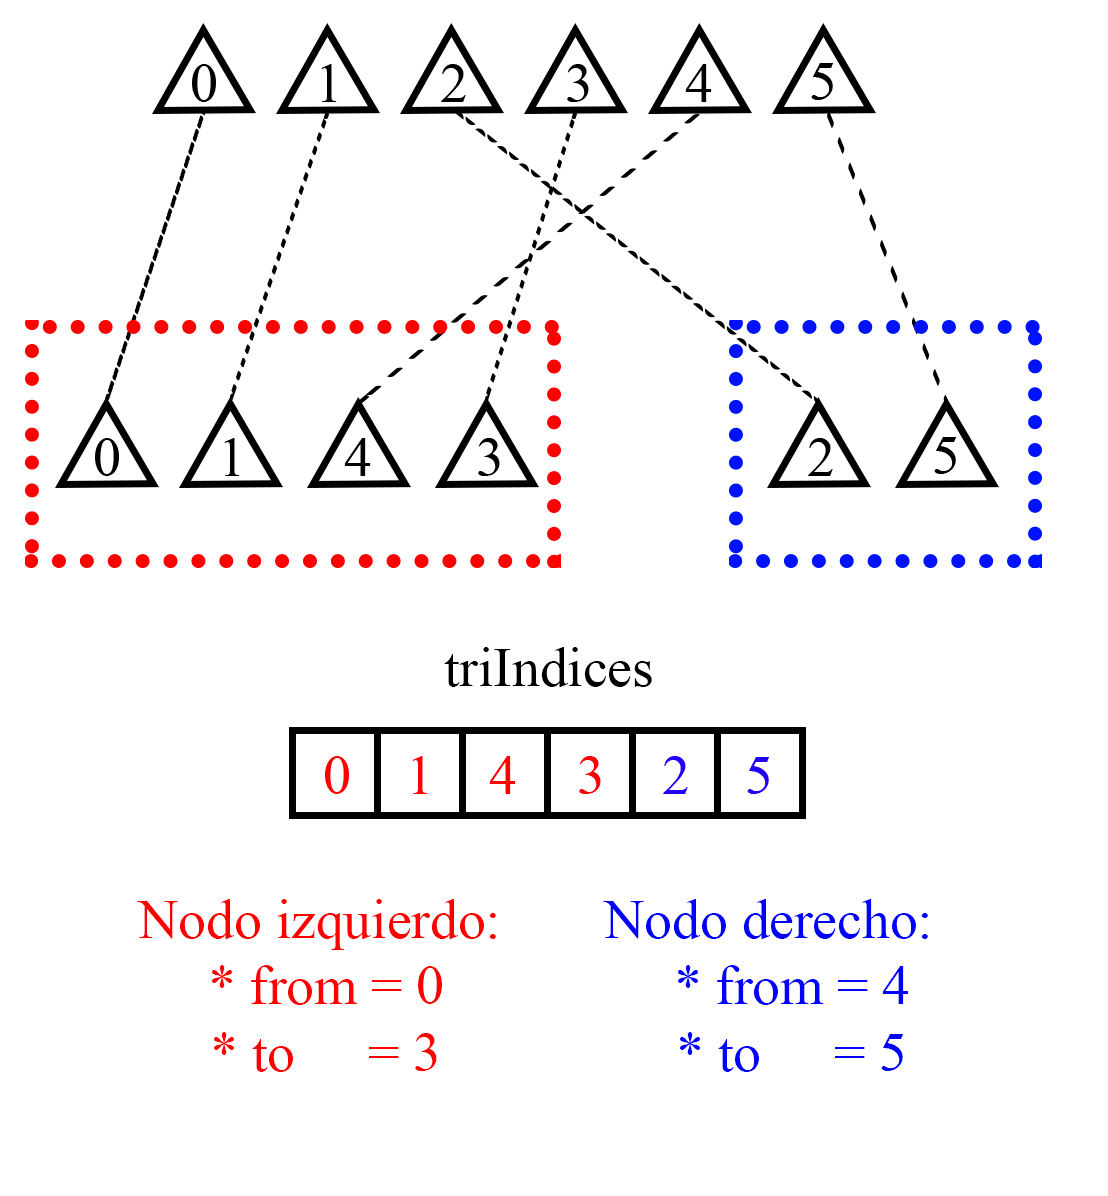
\includegraphics[width=0.4\textwidth]{triIndices}
	\caption{Ejemplo de la ordenación de triángulos a partir de los índices de cada nodo}
	\label{fig:triindices}
\end{figure}

Una vez definida la función de generación de árboles BVH solo queda decidir cómo se van a particionar los triángulos en cada nodo.

El hecho de como separar los nodos hijos de manera óptima no es una tarea trivial, en esta sección se mostrarán comparativas mostrando como los tiempos de recorrido varían dependiendo del método elegido, además de que algunos métodos tardan más en construirse pero permiten recorridos más rápidos mientras que otros métodos permiten la construcción de árboles en tiempo lineal pero no ofrecen tan buenos resultados a la hora de recorrerlos. Estos últimos son más usados en aplicaciones de tiempo real que requieren construir árboles BVH en milisegundos.

La aplicación de este trabajo requiere de varios segundos e incluso minutos por cada escena renderizada, por lo que existe la libertad de construir árboles con métodos más lentos que no afectarán tan negativamente al tiempo total de renderizado.

Se han implementado dos métodos distintos para comparar su rendimiento. Uno de ellos es un método ingenuo y el segundo es un método utilizado en producción conocido como división por heurística de superficie (SAH).

\subsubsection{Partición por plano:}

En el libro Physically based rendering: From theory to implementation \cite{pharr2016physically} se propone un método de partición sencillo. A continuación se explica una interpretación algo distinta de este método que hace uso de los centroides de los triángulos en vez de utilizar el vértice 0 como hace el libro.

Este método no es práctico y se usa tan solo de forma comparativa. Consiste en elegir la dimensión más grande de la caja que envuelve a los triángulos y partirla por la mitad. Posteriormente se recorrerán todos los triángulos y se dividirán por dicho plano. Para saber si un triángulo se encuentra a un lado o al otro se interpretan los triángulos como un punto en el espacio cuya posición es el centroide.

\begin{minipage}[c]{0.95\textwidth}
\begin{lstlisting}[label={cod:planeheuristic}, caption={Heurística de división de plano}]
	
	static void dividePlane(std::vector<BVHTri>* tris, std::vector<BVHTri>* trisLeft, std::vector<BVHTri>* trisRight) {

		Vector3 b1, b2;

		bounds(tris, b1, b2);

		Vector3 l = (b2.x - b1.x, b2.y - b1.y, b2.z - b1.z);

		if (l.x > l.y && l.x > l.z) {

			for (int i = 0; i < tris->size(); i++) {
				if (tris->at(i).tri.centroid().x > b1.x + l.x / 2) {
					trisLeft->push_back(tris->at(i));
				}
				else {
					trisRight->push_back(tris->at(i));
				}
			}

		} else if (l.y > l.x && l.y > l.z) {
			for (int i = 0; i < tris->size(); i++) {
				if (tris->at(i).tri.centroid().y > b1.y + l.y / 2) {
					trisLeft->push_back(tris->at(i));
				}
				else {
					trisRight->push_back(tris->at(i));
				}
			}
		}
		else {
			for (int i = 0; i < tris->size(); i++) {
				if (tris->at(i).tri.centroid().z > b1.z + l.z / 2) {
					trisLeft->push_back(tris->at(i));
				}
				else {
					trisRight->push_back(tris->at(i));
				}
			}
		}
	}
	
\end{lstlisting}
\end{minipage}

\subsubsection{Heurística SAH:}
\label{sub:sah}	

Esta heurística parte de una simplificación en la estimación de tiempo de recorrido para un nodo.

Para un nodo $N$, con $n$ triángulos, se estima que el tiempo en comprobar las intersecciones con cada triángulo es constante $t_{triangulo}$, de manera que el tiempo total para un nodo es $n * t_{triangulo}$. Si este nodo tiene dos hijos, $A$ y $B$, el tiempo en recorrer dicho nodo será $p_A\sum{n_A} + p_B\sum{n_B}$ donde $p$ es la probabilidad de intersecar cada hijo individualmente. La probabilidad de intersecar un nodo se simplifica como el área del volumen delimitador que encierra dicho nodo, de manera que se busca una división de los triángulos que minimice la suma $p_A\sum{n_A} + p_B\sum{n_B}$. El valor de esta suma es la denominada \code{SAH} y como se ha concluído que estima el tiempo de recorrido de un nodo, es necesario construir un árbol BVH para el cual sus nodos cuenten con un valor mínimo de esta estimación de tiempo de recorrido.

Dicho esto, buscar una división de los triángulos que minimicen la fórmula propuesta sería una tarea sencilla si se probara cada combinación de triángulos. No hace falta decir que es inviable comprobar todas las combinaciones para escenas del orden de millones de triángulos, por lo que es necesario aplicar otra simplifiación adicional. Esta simplificación se propone en \cite{wald2007fast}, donde Wald la denomina ''bining''. Por otro lado, PBRT \cite{pharr2016physically} describe esta misma simplificación utilizando el término ''buckets''.

La técnica de ''bining'' se aplica para cada dimensión individualmente. Se divide un nodo en \code{BVH\_SAHBINS} partes iguales y cada una de estas divisiones se considera un ''bin''. Para todos los triángulos, se calcula el ''bin'' en el que se encuentran (utilizando su centroide como punto de división) y se añaden a este. Añadir un triángulo a un ''bin'' significa incrementar la cuenta de triángulos en dicho ''bin'' y recalcular el volumen delimitador teniendo en cuenta el nuevo triángulo. Este primer paso se encuentra en la sección del código \code{//Bin initialization}.

En la figura \autoref{fig:binning} se ejemplifica el primer procedimiento, el contenedor 1 tiene la suma de 2 triángulos y el volumen delimitador asociado $BB1$ mientras que los contenedores 3 y 5 solo cuentan con un triángulo y sus volúmenes delimitadores son $BB3$ y $BB5$ respectivamente.

\begin{figure}[H]
    \centering
	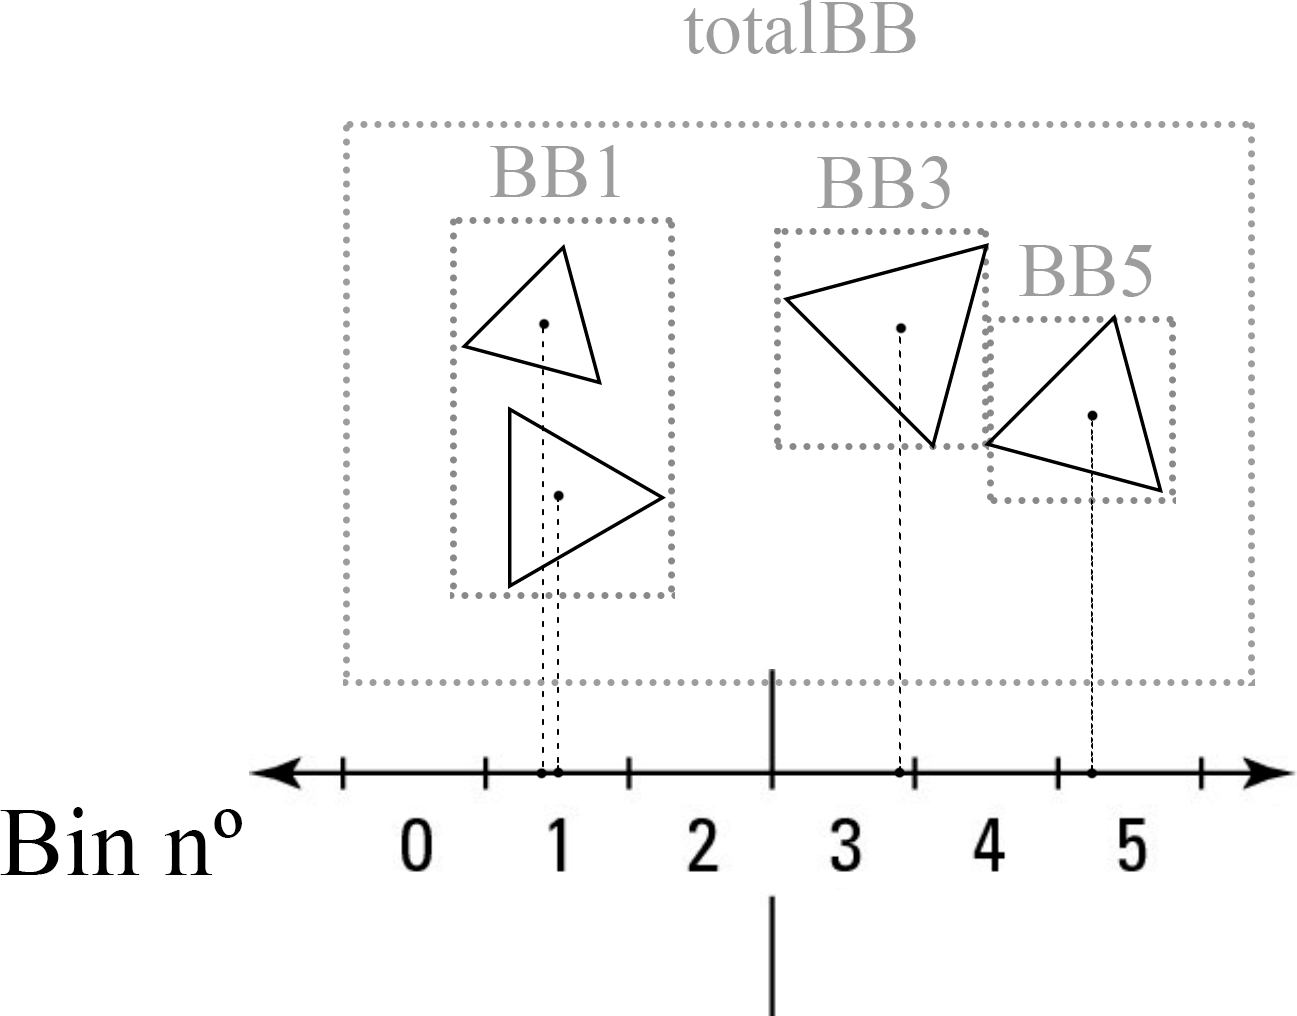
\includegraphics[width=0.5\textwidth]{binning}
	\caption{Relleno de ''bins''}
	\label{fig:binning}
\end{figure}

Se ha explicado como se clasifican los triángulos en contenedores, pero queda pendiente la manera en la que se aprovecha esta clasificación. Se crean \code{BVH\_SAHBINS} nodos hipotéticos. Cada nodo hipotético representa una división entre los contenedores, determinada por un índice entre 0 y \code{BVH\_SAHBINS} - 1. Dicho nodo hipotético contiene dos hijos: el primero cuenta con la unión de los volúmenes delimitadores y la suma de triángulos de todos los contenedores hasta el índice del nodo hipotético. El segundo es igual pero desde el índice hasta el último contenedor. Esta división se encuentra en la sección del código \code{//Bin filling}.

Por útlimo se procederá a calcular la estimación de tiempo de recorrido para cada nodo hipotético, y el nodo que tenga el valor más bajo, será la división de triángulos que se use.


\begin{lstlisting}[label={cod:sah}, caption={Función de división por SAH}]
	
	static void divideSAH(std::vector<BVHTri>* tris, std::vector<BVHTri>* trisLeft, std::vector<BVHTri>* trisRight) {

		if (tris->size() <= 0)
			return;

		Vector3 totalB1, totalB2;

		int bestBin = 0;
		int bestAxis = 0;
		float bestHeuristic = std::numeric_limits<float>::max();

		bounds(tris, totalB1, totalB2);

		for (int axis = 0; axis < 3; axis++) {

			Vector3 b1s[BVH_SAHBINS];
			Vector3 b2s[BVH_SAHBINS];

			int count[BVH_SAHBINS];

			// Bin initialization
			for (int i = 0; i < BVH_SAHBINS; i++) {
				count[i] = 0;
				b1s[i] = Vector3();
				b2s[i] = Vector3();
			}

			// Bin filling
			for (int i = 0; i < tris->size(); i++) {

				int bin = 0;
				Vector3 b1, b2;

				// The bin which corresponds to certain triangle is calculated
				if (totalB1[axis] != totalB2[axis]) {
					float c = tris->at(i).tri.centroid()[axis];
					bin = map(c, totalB1[axis], totalB2[axis], 0, BVH_SAHBINS - 1);
				}

				count[bin]++;
				bounds(tris->at(i).tri, b1, b2);
				boundsUnion(b1s[bin], b2s[bin], b1, b2, b1s[bin], b2s[bin]);
			}
			
			for (int i = 0; i < BVH_SAHBINS; i++) {

				// Tris in the first and second child
				int count1 = 0;	int count2 = 0;

				// b1, b2 are the boundings for first child, b3, b4 for the second one
				Vector3 b1, b2, b3, b4;

				// First swept for first child from 0 to i
				for (int j = 0; j < i; j++) {
					count1 += count[j];
					boundsUnion(b1, b2, b1s[j], b2s[j], b1, b2);
				}

				// Second swept for second child from i to BVH_SAHBINS - 1
				for (int k = i; k < BVH_SAHBINS; k++) {
					count2 += count[k];
					boundsUnion(b3, b4, b1s[k], b2s[k], b3, b4);
				}

				float heuristic = boundsArea(b1, b2) * (float)count1 + boundsArea(b3, b4) * (float)count2;

				if (heuristic < bestHeuristic) {
					bestHeuristic = heuristic;
					bestBin = i;
					bestAxis = axis;
				}
			}
		}
		
		// Tri division depending on the bin
		for (int i = 0; i < tris->size(); i++) {

			float c = tris->at(i).tri.centroid()[bestAxis];
			int bin = map(c, totalB1[bestAxis], totalB2[bestAxis], 0, BVH_SAHBINS - 1);

			if (bin < bestBin) {
				trisLeft->push_back(tris->at(i));
			}
			else {
				trisRight->push_back(tris->at(i));
			}
		}
	}

\end{lstlisting}
	

\subsection{Operación de recorrido (GPU)}
	
El recorrido de árboles es una tarea intuitivamente recursiva y cuenta con una implementación conocida y sencilla. No obstante la recursión es un proceso indeseado en CUDA debido a las pilas relativamente pequeñas de los dispositivos de aceleración gráfica. Así pues también generan una divergencia superior, un proceso con alta penalización en el rendimiento.

Para demostrar esto se ha hecho uso de dos implementaciones de la función de recorrido. La primera es una función recursiva de recorrido de árboles binarios:

\begin{minipage}[c]{0.95\textwidth}
\begin{lstlisting}[label={cod:bvhtransversalrec}, caption={Recorrido del árbol BVH recursivo}]
	
	__host__ __device__ void transverseAux(Ray ray, Hit& nearestHit, Node& node) {
	
		if (node.depth == BVH_DEPTH) {
			intersectNode(ray, node, nearestHit);
			return;
		}
	
		Node lChild = leftChild(node.idx, node.depth);
		Node rChild = rightChild(node.idx, node.depth);
	
		if (intersect(ray, lChild.b1, lChild.b2))
			transverseAux(ray, nearestHit, lChild);
		
		if (intersect(ray, rChild.b1, rChild.b2))
			transverseAux(ray, nearestHit, rChild);		
	}

\end{lstlisting}
\end{minipage}
	
Karras explica en el blog de desarrolladores de Nvidia \cite{karrastransversal} cómo usar las estructuras BVH para detectar colisiones físicas entre objetos en la GPU. Así pues, la segunda implementación viene dada a partir de ciertas modificaciones al código de recorrido propuesto, donde se puede adaptar a un caso más específico como es la intersección de Rayo \- BVH necesaria en Eleven Renderer. Esta implementación rompe con la recursividad a partir de una pila de nodos, quedando así una función iterativa.

\begin{minipage}[c]{0.95\textwidth}
\begin{lstlisting}[label={cod:bvhtransversalit}, caption={Recorrido del árbol BVH iterativo}]
		
	__device__ void transverse(Ray ray, Hit& nearestHit) {

		Node stack[64];

		Node* stackPtr = stack;

		(*stackPtr++).valid = false;

		Node node = nodes[0];

		do {

			Node lChild = leftChild(node.idx, node.depth);
			Node rChild = rightChild(node.idx, node.depth);

			bool lOverlap = intersect(ray, lChild.b1, lChild.b2);
			bool rOverlap = intersect(ray, rChild.b1, rChild.b2);

			if (node.depth == (BVH_DEPTH - 1) && rOverlap)
				intersectNode(ray, rChild, nearestHit);

			if (node.depth == (BVH_DEPTH - 1) && lOverlap)
				intersectNode(ray, lChild, nearestHit);
			
			bool traverseL = (lOverlap && node.depth != (BVH_DEPTH - 1));
			bool traverseR = (rOverlap && node.depth != (BVH_DEPTH - 1));

			if (!traverseL && !traverseR) {
				node = *--stackPtr;

			} else {
				node = (traverseL) ? lChild : rChild;
				if (traverseL && traverseR)
					*stackPtr++ = rChild;
			}

		} while (node.valid);
	}
	
\end{lstlisting}
\end{minipage}

Una breve evaluación de ambas funciones muestran una clara ventaja en la implementación iterativa. Además ha sido necesario limitar la profundidad a 6 nodos debido a las limitaciones mencionadas anteriormente. El uso de más profundidad en el entorno utilizado provoca el bloqueo del kernel

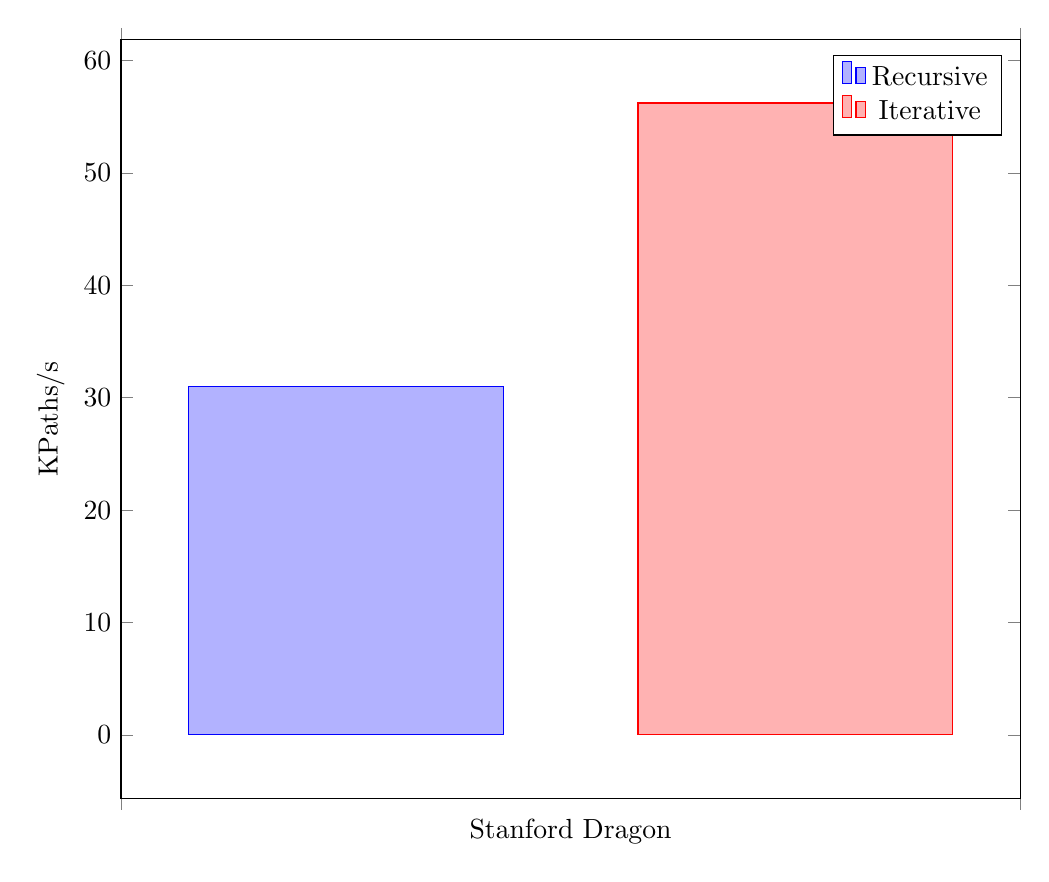
\begin{tikzpicture}
	\begin{axis}[
	x tick label style={
		/pgf/number format/1000 sep=},
	ylabel=KPaths/s,
	width=13cm,
	enlarge x limits=-1,
	ybar interval=0.7,
	symbolic x coords={Suzanne,Stanford Bunny,Stanford Dragon, test}
]
\addplot 
	coordinates {(Stanford Dragon,31.03) (test,0)};
\addplot 
	coordinates {(Stanford Dragon,56.23) (test,0)};
\legend{Recursive,Iterative}
\end{axis}
\end{tikzpicture}


	
\subsubsection{Comparación de heurísticas:}
	
Para justificar el uso de la heurística por superficie de área se muestra una ejecución de ambas heurísticas con tres modelos ampliamente utilizados en evaluaciones comparativas de computación gráfica:

\begin{itemize}
	
	\item Suzanne: 968 triángulos
	\item Stanford Bunny: 4968 triángulos
	\item Stanford Dragon: 871306 triángulos
	
\end{itemize}

\begin{tabular}{ |p{3cm}||p{3cm}|p{3cm}| }
	 \hline
	 \multicolumn{3}{|c|}{Heuristic comparaison: Build time\footnotemark} \\
	 \hline
	 Model Name&PD\footnotemark build time&SAH build time\\
	 \hline
	 Suzanne   &68ms&93ms\\
	 Stanford Bunny &70ms&205ms\\
	 Stanford Dragon &3490ms&5647ms\\
	 \hline
\end{tabular}

\begin{tabular}{ |p{3cm}||p{3cm}|p{3cm}| }
	 \hline
	 \multicolumn{3}{|c|}{Heuristic comparaison: Transversal efficiency} \\
	 \hline
	 Model Name&PD transversal eff&SAH transversal eff\\
	 \hline
	 Suzanne   &2829 kPath/s&13073 kPath/s\\
	 Stanford Bunny &553 kPath/s&14153 kPath/s\\
	 Stanford Dragon &1.78 kPath/s&11587 kPath/s\\
	 \hline
\end{tabular}

\footnotetext{Evaluaciones llevadas a cabo en una GPU NVIDIA RTX 3090 y un procesador Intel i5 6600K}
\footnotetext{PD = Plane Division}

\begin{figure}[H]
	\centering
  \begin{minipage}[b]{0.4\textwidth}
    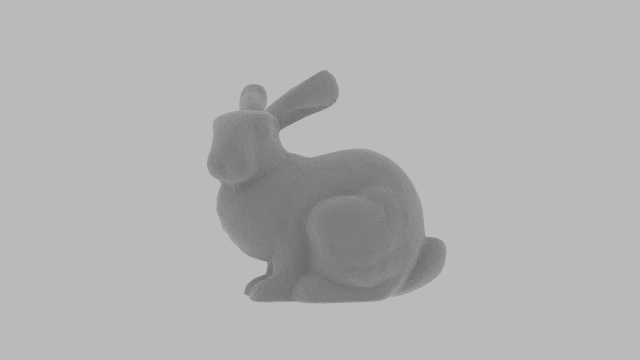
\includegraphics[width=\textwidth]{bunny}
    \caption{Stanford Bunny.}
  \end{minipage}
  \hfill
  \begin{minipage}[b]{0.4\textwidth}
    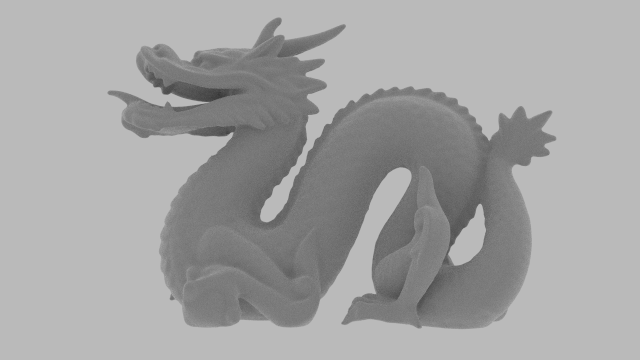
\includegraphics[width=\textwidth]{dragon}
    \caption{Stanford Dragon.}
  \end{minipage}
\end{figure}

Tras el análisis de ambas heurísticas en distintas escenas, se concluye que el tiempo de generación de árboles BVH es significativamente más lento con SAH para escenas complejas. Por otro lado, la heurística de división de plano tiene un rendimiento de recorrido nefasto hasta el punto de ser inservible para escenas del orden de cientos de miles de triángulos.
	
\subsection{Evaluación:}
	
Finalmente es necesario elegir los parámetros para \code{BVH\_DEPTH} y \code{SAH\_BINS}. Puesto que existen varios tipos de escenas con distintas geometrías, se va a dejar de lado cualquier tipo de enfoque analítico y se va a hacer uso de medidas en casos reales. Se procede a realizar una evaluación con distintos parámetros.
	
En el caso de la selección de \code{SAH\_BINS}, Indigo Wald propone 16 como límite \cite{wald2007fast} debido a la insustancial mejora de rendimiento para valores mayores. Esto se ha podido comprobar directamente en Eleven Renderer donde se ha llevado a cabo la construcción y recorrido de BVH para la escena "Stanford Dragon" variando la cantidad de contenedores \autoref{fig:sahbins}. Se comprueba que la velocidad de recorrido se estanca para los valores 12-16, mientras que el tiempo de generación permanece lineal. Eleven Render utiliza de manera predeterminada \code{SAH\_BINS = 14} tras el análisis realizado.

\begin{figure}[H]
\centering
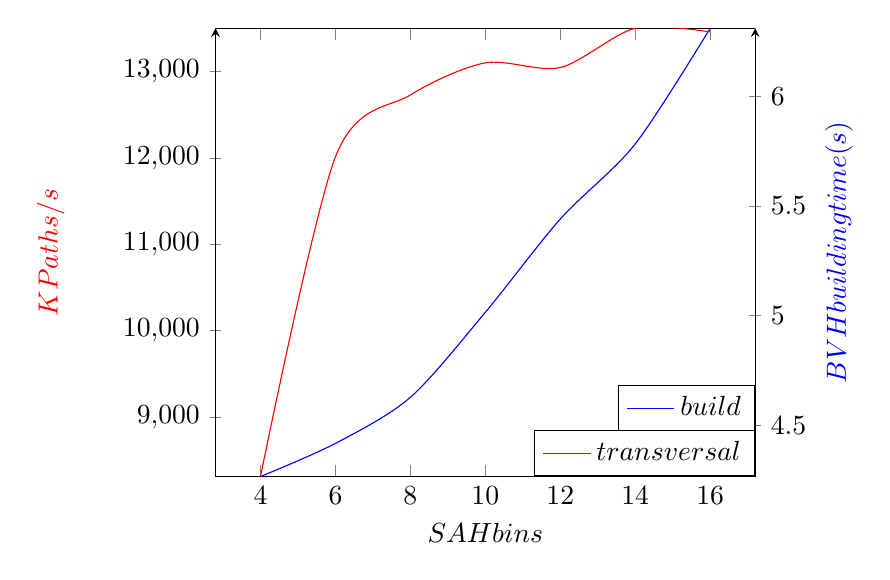
\begin{tikzpicture}

\begin{axis}[
    axis y line = right,
    xlabel = \(SAH bins\),
    ylabel = {\(\textcolor{blue}{BVH building time (s)}\)},
	legend style={at={(1,0.1)},anchor=south east},
	scaled y ticks=false
]

\addplot[smooth, blue]
coordinates{(4,4.267) (6, 4.418) (8, 4.628) (10, 5.015) (12, 5.440) (14, 5.782) (16, 6.309)};
\addlegendentry{\(build\)}
\end{axis}

\begin{axis}[
    axis y line = left,
	axis x line = none,
    xlabel = \(SAH bins\),
    ylabel = {\(\textcolor{red}{KPaths/s}\)},
	ylabel style={yshift=0.5cm},
	legend style={at={(1,0)},anchor=south east},
	scaled y ticks=false
]

\addplot [smooth, red]
coordinates{(4,8310) (6, 12012) (8, 12728) (10, 13100) (12, 13046) (14, 13501) (16, 13458)};
\addlegendentry{\(transversal\)}

\end{axis}
\end{tikzpicture}
\caption{Comparación de tiempos de construcción y eficiencia de recorrido para distinto número de contenedores}
\label{fig:sahbins}
\end{figure}